Lo scopo di questa esperienza è la valutazione dell'effetto delle \textbf{correnti di bias} sulle prestazioni di un circuito integratore. Per questo esperimento si è  scelto l’amplificatore operazione 1458, dal momento che ha una corrente di bias piuttosto elevata (questo di solito è un considerato un difetto, specialmente se si realizzano circuiti integratori). Il circuito è riportato in Figura \ref{fig:Circuit4}
Sono stati utilizzati i seguenti componenti:
\begin{itemize}
    \item Amplificatore operazionale 1458, codice MC1458
    \item Condensatore a film $C=100nF$
    \item Resistenza $R=330\text{k}\Omega$, 
    \item Interruttore a bottone FSM2JART
\end{itemize}
\begin{figure}[H]
    \centering
    
\includegraphics[width=0.45\linewidth]{images/Circuit4.png}
    \caption{Schema circuito}
    \label{fig:Circuit4}
\end{figure}
Il circuito è alimentato dalla tensione duale $\pm V_{CC}=\pm 10V$.
\subsection{Analisi del datasheet}
Sulla base delle informazioni contenute nel datasheet del 1458, si è ricavata la corrente di bias tipica
\begin{equation*}
    I_{bias}=80nA
\end{equation*}
\clearpage
\subsection{Procedure e risultati}
Abbiamo connesso un multimetro digitale all'uscita $V_{out}$, come si vede in Figura \ref{fig:LabCircuit4}
\begin{figure}[H]
    \centering
    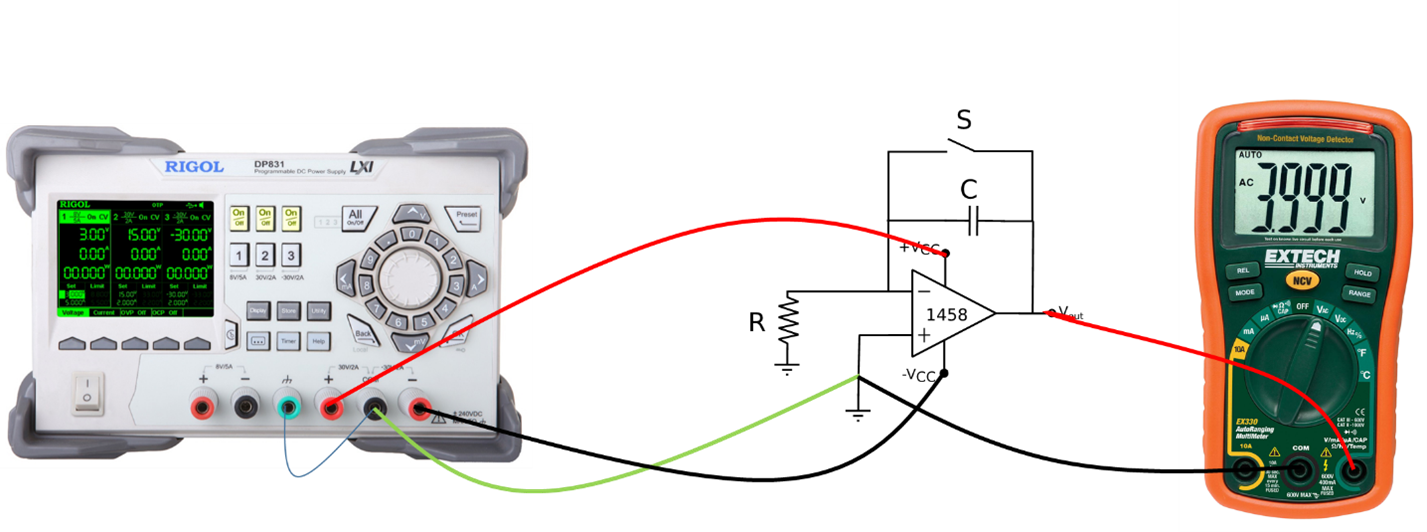
\includegraphics[width=0.8\linewidth]{images/LabCircuit4.png}
    \caption{Schema di collegamento del circuito in Figura \ref{fig:Circuit4}}
    \label{fig:LabCircuit4}
\end{figure}
Durante il controllo preliminare, con il circuito disalimentato e la capacità C scarica, è risultata una lettura di 0V sul multimetro.\\ 
Una volta alimentato, data la non idealità dell'amplificatore operazionale, la tensione di uscita $V_{out}$ ha mostrato un aumento lineare nel tempo fino alla saturazione. Questo effetto è dovuto alla corrente di bias che viene integrata dall'operazionale, generando una cauta di tensione sul condensatore C.\\
Premendo l'interruttore S è possibile scaricare il condensatore; invece quando l'interruttore viene rilasciato riparte il processo di integrazione della corrente di bias.\\\\
Partendo dallo stato di capacità C scarica, al rilascio dell'interruttore si fa partire un cronometro e lo si ferma quando il valore della tensione di uscita ha raggiunto $2.5V$.
Si è deciso di compiere 5 misure di tempo e di svolgere la media in modo da avere un risultato più accurato.
\begin{equation}
    t(V_{out}=2.5V)=13.72s
\end{equation}
Successivamente è stata stimata la corrente di bias dell'amplificatore operazionale
\begin{equation}
    I_{Bias}=18.22nA
\end{equation}
Il calcolo è stato svolto utilizzando la relazione tensione-corrente del condensatore 
\begin{equation}
    i(t)=C\frac{dv}{dt}\implies I_{Bias}=C\frac{V}{t}
\end{equation}
Tale valore si discosta dal valore fornito dal produttore in quanto nel datasheet è fornita la corrente di bias tipica al caso peggiore.
\clearpage
\subsubsection{Risultati in seguito all'aggiunta di un resistore al morsetto non invertente}
Come si vede dalla Figura \ref{fig:Circuit4.1} è stato aggiunto un secondo resistore al morsetto non invertente, con lo scopo di ridurre significativamente l'effetto della corrente di bias.
\begin{figure}[H]
    \centering
    
\includegraphics[width=0.4\linewidth]{images/Circuit4.1.png}
    \caption{Schema circuito con resistenza al morsetto non invertente}
    \label{fig:Circuit4.1}
\end{figure}
\begin{figure}[H]
    \centering
    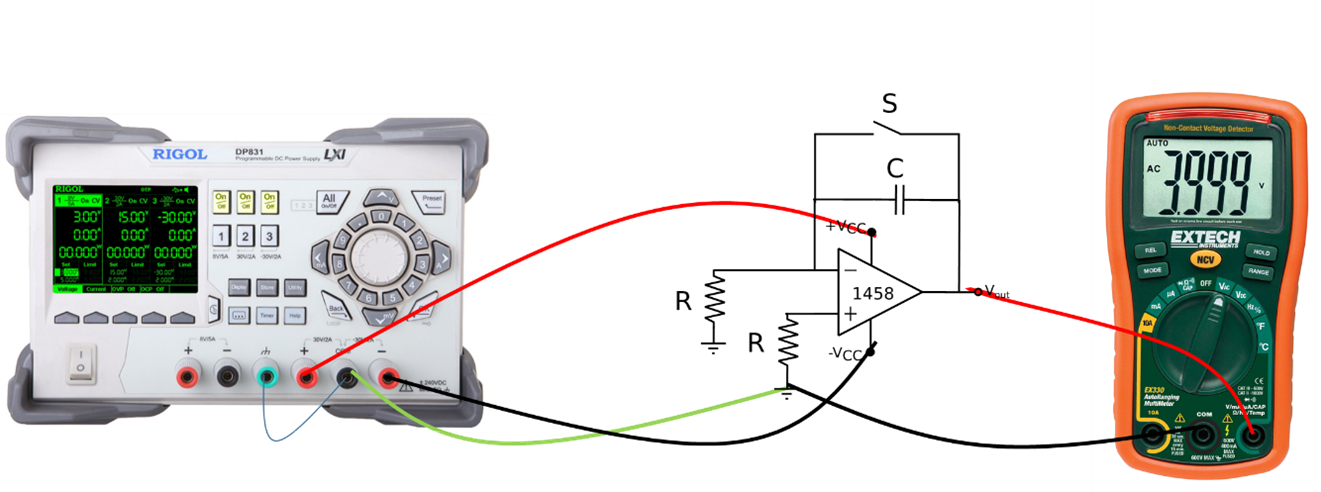
\includegraphics[width=0.7\linewidth]{images/LabCircuit4.1.png}
    \caption{Schema di collegamento del circuito in Figura \ref{fig:Circuit4.1}}
    \label{fig:LabCircuit4.1}
\end{figure}
Ripetendo la modalità di misurazione del punto precedente si è osservato che la tensione aveva un andamento decrescente, non arrivando di fatto mai al valore di 2.5V. Questo è dovuto sempre alle asimmetrie dell'operazionale e quindi ad una corrente $I_{OS}$ negativa.